La integración contínua es una disciplina que permite automatizar el flujo de código desde el momento en que un desarrollador lo genera hasta que llega a la rama principal de código del repositorio, asegurando por el camino que es código de calidad mediante pruebas automáticas mencionadas en las secciones \nameref{section:unit-testing}, \nameref{section:integration-testing} y \nameref{section:e2e-testing}. Además, uniéndolo con el despliegue contínuo, se puede lograr que haciendo solo un click el código sea verificado, enviado a un servidor y expuesto al público. \citet{CVTRVJK} explica este procues en su artículo, mostrando además dos gráficos muy representativos de cómo funcionan la integración contínua (\cref{fig:ci}) y el despliegue contínuo (\cref{fig:cd}).

En la figura \cref{fig:ci} se puede observar cómo múltiples desarrolladores pueden colaborar simultáneamente enviando sus aportaciones a un servidor de control de versiones como GitHub. Mediante un simple evento PUSH en una rama de desarrollo, los cambios irán al repositorio, que emitirá la nueva versión a un servidor de integración contínua. El servidor verificará que el código cubre todos los casos de prueba y, en caso de fracasar, notificará a los desarrolladores involucrados en la nueva versión, que podrán arreglar los fallos y volver a intentar una subida. En caso de éxito, podrá notificar a los desarrolladores también. Sin embargo, lo más habitual es que un éxito desencadene el siguiente proceso, el despliegue contínuo, que se encargará de subir la nueva versión a un servidor público de forma inmediata. Cabe remarcar que este servidor público puede estar duplicado (uno para desarrollo y otro para producción), generando dos procesos de integración contínua que pueden estar tanto encadenados como construidos de forma independiente.

En la figura \cref{fig:cd} se muestra el proceso completo, incluyendo la integración contínua y el despliegue contínuo. En este flujo pueden intervenir revisiones manuales de código y pruebas por parte de los usuarios. Este proceso asume que la aplicación es desarrollada en un entorno profesional, pero el marco que se plantea desarrollar no está pensado en un ámbito de empresa. El marco pretende abarcar proyectos pequeños (de pocos desarrolladores) con potencial de crecer. Por tanto, este flujo debe tenerse en consideración, pero no debe ser la principal preocupación del marco.

La idea es que el marco proporcione de forma sencilla tanto un entorno de integración contínua como un entorno de despliegue contínuo. Es objeto de estudio de este marco analizar las distintas herramientas que permiten hacer estas tareas y pensar en cómo podría un proyecto escalar a ámbito profesional sin modificar las herramientas que se utilizan en el proceso. Para poder realizar estas tareas, se han analizado las dos herramientas gratuitas que propone \citet{CVTRVJK}: Jenkins y CircleCI. TravisCI se descarta por su carácter de pago, que rompe con la filosofía del marco.

\begin{figure}
	\centering
	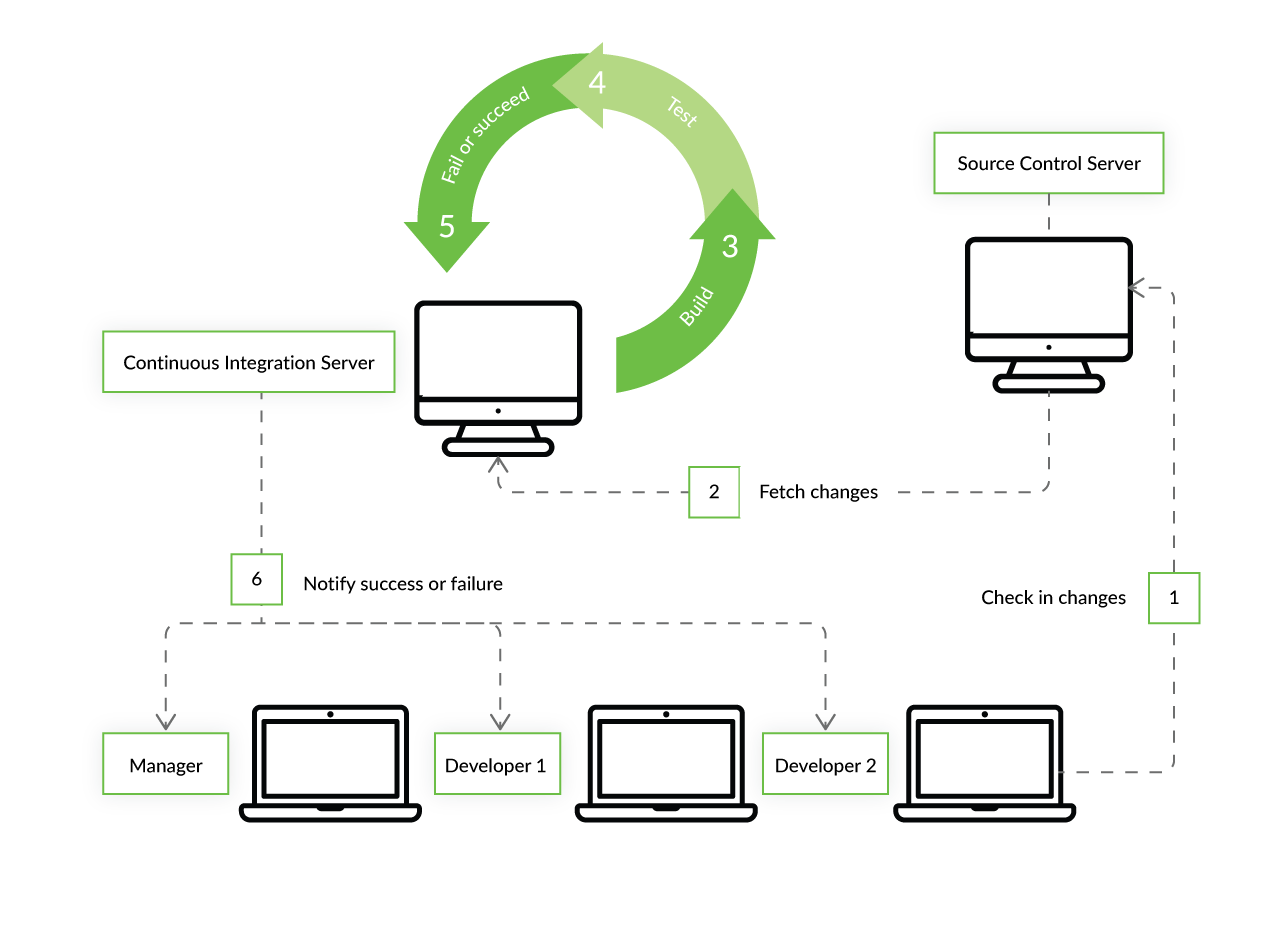
\includegraphics[width=\textwidth]{how-ci-works.png}
	\caption{How Continuous Integration Works}
	\label{fig:ci}
\end{figure}

\begin{figure}
	\centering
	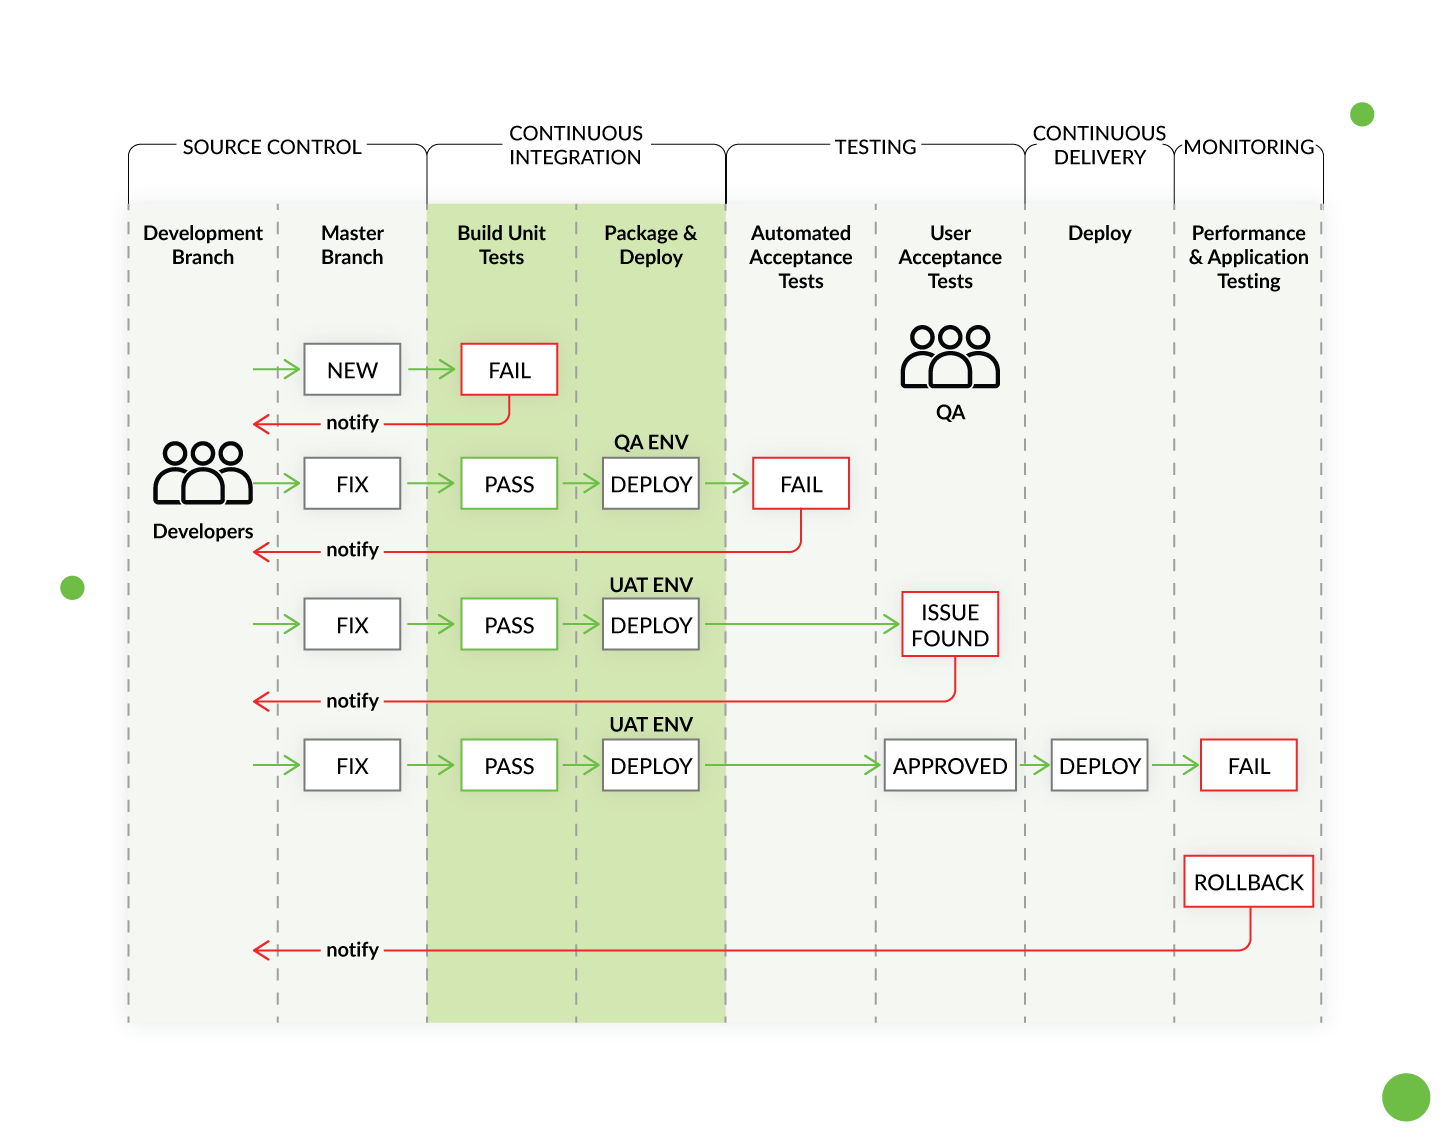
\includegraphics[width=\textwidth]{release-workflow.png}
	\caption{Release Workflow}
	\label{fig:cd}
\end{figure}